\documentclass[a4paper,11pt]{report}

% \sloppy

%%%%%%%%%%%%%%%%%%%%%%%%%%%%%%%%%%%%%%%%%%%%%%%%%%%%%%%%%%%%
% PACKAGES
%%%%%%%%%%%%%%%%%%%%%%%%%%%%%%%%%%%%%%%%%%%%%%%%%%%%%%%%%%%%
\usepackage[utf8]{inputenc}

\usepackage[english]{babel} % francais,

\usepackage{fourier}
% \usepackage{eulervm}
% NOTE: both fourier + eulervm make '<' and '>' not displaid!

\usepackage{pdflscape}

\usepackage{amsmath,amssymb,amsthm,url}
\usepackage{amsfonts}

\usepackage{subcaption}
% \usepackage{marginnote}

\usepackage{longtable}

% \usepackage[pdftex]{graphicx,color}
\usepackage[pdftex,
		colorlinks=true,
% 		pagebackref=true,
		citecolor=darkgreen,
		linkcolor=darkblue,
		urlcolor=URLCOLOR,
	]{hyperref}

\usepackage{graphicx}
\graphicspath{{./images/}{../logos/}}


% BEGIN Watermarking
\ifdefined\DraftVersion
	\usepackage{draftwatermark}
	\SetWatermarkText{draft}
	\SetWatermarkScale{2}
	\SetWatermarkColor[gray]{0.9}
\fi
% END Watermarking


%%%%%%%%%%%%%%%%%%%%%%%%%%%%%%%%%%%%%%%%%%%%%%%%%%%%%%%%%%%%
% MARGINS, HEADERS AND FOOTERS
%%%%%%%%%%%%%%%%%%%%%%%%%%%%%%%%%%%%%%%%%%%%%%%%%%%%%%%%%%%%

\usepackage[top=1cm,bottom=2.5cm,includeheadfoot,headheight=2.5cm,\ifdefined\DraftVersion showframe \else\fi]{geometry}

% \setlength{\parskip}{1ex}

\usepackage{fancyhdr}
\pagestyle{fancy}

% Reset headers and footers
% \fancyhf{}

% Reset header but not footer
\fancyhead{}

\fancyhead[l]{%
	\titleOnHeader{}
}

\fancyhead[r]{%
	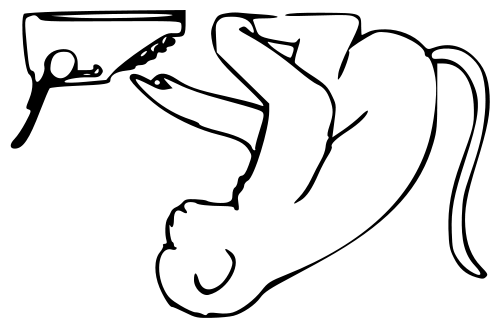
\includegraphics[height=1em]{../logos/imitator-500.png}
	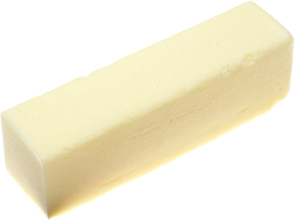
\includegraphics[height=1em]{../logos/logo2-300.png}
	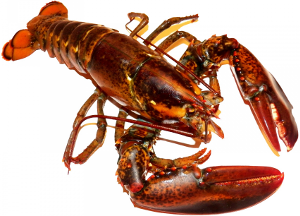
\includegraphics[height=1em]{../logos/logo2-12-300.png}
}

\renewcommand{\headrulewidth}{.1pt}
\renewcommand{\footrulewidth}{0pt}

% \fancyfoot[c]{}
% \fancyfoot[R]{\footnotesize{\thepage}}



%%%%%%%%%%%%%%%%%%%%%%%%%%%%%%%%%%%%%%%%%%%%%%%%%%%%%%%%%%%%
% TIKZ
%%%%%%%%%%%%%%%%%%%%%%%%%%%%%%%%%%%%%%%%%%%%%%%%%%%%%%%%%%%%
\usepackage[svgnames,table]{xcolor}

\usepackage{pgf}
\usepackage{tikz}
\usetikzlibrary{arrows,automata,decorations.pathmorphing}
% Couleurs

\definecolor{darkblue}{rgb}{0.0,0.0,0.6}
\definecolor{darkgreen}{rgb}{0, 0.5, 0}
\definecolor{URLCOLOR}{rgb}{.4, .4, .7}


\definecolor{turquoise}{rgb}{0 0.41 0.41}
\definecolor{rouge}{rgb}{0.79 0.0 0.1}
\definecolor{vert}{rgb}{0.15 0.4 0.1}
\definecolor{mauve}{rgb}{0.6 0.4 0.8}
\definecolor{violet}{rgb}{0.58 0. 0.41}
\definecolor{orange}{rgb}{0.8 0.4 0.2}
\definecolor{bleu}{rgb}{0.39, 0.58, 0.93}
\definecolor{gris}{rgb}{0.6,0.6,0.6}
\definecolor{grisfonce}{rgb}{0.4,0.4,0.4}
% Jeu de couleurs pales
\definecolor{cpale1}{rgb}{1, 0.3, 0.3}
\definecolor{cpale2}{rgb}{0.3, 1, 0.3}
\definecolor{cpale3}{rgb}{0.3, 0.3, 1}
\definecolor{cpale4}{rgb}{1, 0.3, 1}
\definecolor{cpale5}{rgb}{1, 1, 0.3}
\definecolor{cpale6}{rgb}{0.3, 1, 1}
\definecolor{cpale7}{rgb}{0.9, 0.6, 0.2}
\definecolor{cpale8}{rgb}{0.7, 0.4, 1}
\definecolor{cpale9}{rgb}{0.5, 1, 0.75}
\definecolor{cpale10}{rgb}{0.8, 0.7, 0.6}
\definecolor{cpale11}{rgb}{0.6, 0.7, 0.8}
\definecolor{cpale12}{rgb}{0.2, 0.5, 0.9}
\definecolor{cpale13}{rgb}{0.5, 0.9, 0.2}
\definecolor{cpale14}{rgb}{0.9, 0.2, 0.5}
\definecolor{cpale15}{rgb}{0.7, 0.7, 0.7}
\definecolor{cpale16}{rgb}{0.8, 0.8, 0.5}


%%%%%%%%%%%%%%%%%%%%%%%%%%%%%%%%%%%%%%%%%%%%%%%%%%%%%%%%%%%%
% CLEVER REFERENCES
%%%%%%%%%%%%%%%%%%%%%%%%%%%%%%%%%%%%%%%%%%%%%%%%%%%%%%%%%%%%
\usepackage[capitalise,english,nameinlink]{cleveref} % load after algorithm2e and hyperref
% \crefname{line}{\text{line}}{\text{lines}} % to remove the capital


%%%%%%%%%%%%%%%%%%%%%%%%%%%%%%%%%%%%%%%%%%%%%%%%%%%%%%%%%%%%
% CONSTANTS
%%%%%%%%%%%%%%%%%%%%%%%%%%%%%%%%%%%%%%%%%%%%%%%%%%%%%%%%%%%%
%-%-%-%-%-%-%-%-%-%-%-%-%-%-%-%-%-%-%-%-%-%-%-%-%-%-%-%-%-%
% MATHS
%-%-%-%-%-%-%-%-%-%-%-%-%-%-%-%-%-%-%-%-%-%-%-%-%-%-%-%-%-%
% Variables
\def\init{\ensuremath{\textsf{init}}} % \xspace
\newcommand{\A}{\mathcal{A}}
\newcommand{\Action}{\ensuremath{\Sigma}}
\newcommand{\action}{a}
\newcommand{\ArithExpr}{\mathcal{AE}} % (#1)% set of all constraints over some set
\newcommand{\ArithExprD}{\ArithExpr(\DVar)}
\newcommand{\C}{C}
\newcommand{\Cinit}{\C_\init} % initial constraint
\newcommand{\Clock}{X} % set of clocks
\newcommand{\ClockCard}{H} % cardinality of clocks
\newcommand{\clock}{x} % clock
\newcommand{\clockval}{w} % clock valuation
\newcommand{\Cupdates}{\Clock_\mathsf{up}}
\newcommand{\Dupdates}{\DVar_\mathsf{up}}
\newcommand{\dval}{\ensuremath{\delta}} % discrete variable
\newcommand{\DVar}{D} % set of discrete variables
\newcommand{\dvar}{d} % discrete variable
\newcommand{\DVarCard}{J} % cardinality of discrete variables
% \newcommand{\DVarinit}{\DVar_\init} % discrete variable
\newcommand{\edge}{e}
\newcommand{\guard}{g}
\newcommand{\invariant}{I}
\newcommand{\LConstraint}{\mathcal{LC}} % (#1)% set of all constraints over some set
\newcommand{\LConstraintD}{\LConstraint(\DVar)}
\newcommand{\LConstraintXP}{\LConstraint(\Clock \cup \Param)}
\newcommand{\LConstraintXPD}{\LConstraint(\Clock \cup \Param \cup \DVar)}
\newcommand{\lterm}{\mathit{lt}}
\newcommand{\LTerm}{\mathcal{LT}} % (#1)% set of all linear terms over some set
\newcommand{\LTermD}{\LTerm(\DVar)}
\newcommand{\LTermXPD}{\LTerm(\Clock \cup \Param \cup \DVar)}
\newcommand{\loc}{\ell} % location
\newcommand{\locinit}{\loc_\init}
\newcommand{\Loc}{L} % set of locations
\newcommand{\Param}{P} % set of parameters
\newcommand{\param}{p} % parameter
\newcommand{\ParamCard}{M} % number of parameters
\newcommand{\pval}{v} % parameter valuation
% \newcommand{\resets}{R}
\newcommand{\steps}{ {\rightarrow} }
\newcommand{\stopwatches}{S}
\newcommand{\tuple}[1]{\langle#1\rangle}
\newcommand{\unobs}{\ensuremath{\epsilon}}
\newcommand{\Var}{\mathit{Var}} % set of variables
\newcommand{\var}{\mathit{z}} % variable
\newcommand{\VarCard}{N} % cardinality of variables % TODO: conflict

% Ensembles
\newcommand{\grandb}{{\mathbb B}}
\newcommand{\grandn}{{\mathbb N}}
\newcommand{\grandq}{{\mathbb Q}}
\newcommand{\grandqplus}{{\mathbb Q}_{\geq 0}}
\newcommand{\grandr}{{\mathbb R}}
\newcommand{\grandrplus}{\grandr_{\geq 0}}
\newcommand{\grandz}{{\mathbb Z}}

% Unites
\newcommand{\micros}{\mathit{\mu s}}
\newcommand{\nanos}{ns}

% Noms
\newcommand{\tiling}{\mathit{Tiling}}
% \newcommand{\true}{\mathbf{true}}
\newcommand{\Ko}{K}
\newcommand{\pio}{\pi_0}
\newcommand{\piprime}{\pi}
\newcommand{\To}{T_0}
\newcommand{\Tprime}{T}

% Symboles
\newcommand{\emptystring}{$\epsilon$}
\newcommand{\fleche}[1]{\stackrel{#1}{\rightarrow}}
\newcommand{\Fleche}[1]{\stackrel{#1}{\Rightarrow}}
% \newcommand{\steps}[0]{ {\rightarrow} }

% Booleens
\newcommand{\false}{{\tt false}}
\newcommand{\true}{{\tt true}}

% PARAMETRES RCP
\newcommand{\rcpFMax}{\mathit{rc\_fast\_max}}
\newcommand{\rcpFMin}{\mathit{rc\_fast\_min}}
\newcommand{\rcpSMax}{\mathit{rc\_slow\_max}}
\newcommand{\rcpSMin}{\mathit{rc\_slow\_min}}
\newcommand{\rcpD}{\mathit{delay}}

%-%-%-%-%-%-%-%-%-%-%-%-%-%-%-%-%-%-%-%-%-%-%-%-%-%-%-%-%-%
% ALGORITHMES
%-%-%-%-%-%-%-%-%-%-%-%-%-%-%-%-%-%-%-%-%-%-%-%-%-%-%-%-%-%
% Algorithmes PTA
\newcommand{\BC}{\ensuremath{\mathsf{BC}}}
\newcommand{\EFsynth}{\ensuremath{\mathsf{EFsynth}}}
\newcommand{\IM}{\ensuremath{\mathsf{IM}}}
\newcommand{\PDFC}{\ensuremath{\mathsf{PDFC}}}
\newcommand{\PRP}{\ensuremath{\mathsf{PRP}}}
\newcommand{\PRPC}{\ensuremath{\mathsf{PRPC}}}


%-%-%-%-%-%-%-%-%-%-%-%-%-%-%-%-%-%-%-%-%-%-%-%-%-%-%-%-%-%
% CONSTANTES DE CHAINES
%-%-%-%-%-%-%-%-%-%-%-%-%-%-%-%-%-%-%-%-%-%-%-%-%-%-%-%-%-%

% Outils
% \newcommand{\apron}{\textsc{Apron}}
\newcommand{\CosyVerif}{\emph{CosyVerif}}
\newcommand{\gdot}{\texttt{dot}}
\newcommand{\graphviz}{Graphviz}
\newcommand{\hytech}{{\sc HyTech}}
\newcommand{\imitator}{\textsf{IMITATOR}}
\newcommand{\imitatorExec}{\code{imitator}}
\newcommand{\IPTA}{IPTA}
\newcommand{\NIPTA}{NIPTA}
\newcommand{\ocaml}{OCaml}
\newcommand{\pat}{PAT}
\newcommand{\phaver}{PHAVer}
\newcommand{\phaverLite}{PHAVerLite}
% \newcommand{\polka}{NewPolka}
% \newcommand{\prism}{\textsc{Prism}}
% \newcommand{\red}{RED}
\newcommand{\uppaal}{\textsc{Uppaal}}

\newcommand{\binimitator}{./imitator}


% Current version
\newcommand{\imitatorversion}{2.12}
\newcommand{\imitatorversionname}{Butter Lobster}


%%%%%%%%%%%%%%%%%%%%%%%%%%%%%%%%%%%%%%%%%%%%%%%%%%%%%%%%%%%%
% THEOREMS
%%%%%%%%%%%%%%%%%%%%%%%%%%%%%%%%%%%%%%%%%%%%%%%%%%%%%%%%%%%%
\usepackage[framemethod=TikZ]{mdframed}

%------------------------------------------------------------
\theoremstyle{plain}
%------------------------------------------------------------


%------------------------------------------------------------
\theoremstyle{definition}
%------------------------------------------------------------
\newtheorem{mydefinition}{Definition}[chapter]
\newenvironment{definition}%
	{\begin{mdframed}[roundcorner=3pt,backgroundcolor=blue!7,linecolor=blue!70,linewidth=2]\begin{mydefinition}}
	{\end{mydefinition}\end{mdframed}}

\newtheorem{myexample}{Example}[chapter]
\newenvironment{example}
	{\begin{mdframed}[roundcorner=3pt,backgroundcolor=green!7,linecolor=green!70,linewidth=2]\begin{myexample}}
	{\end{myexample}\end{mdframed}}

%------------------------------------------------------------
\theoremstyle{remark}
%------------------------------------------------------------
\newtheorem{myremark}{Remark}[chapter]
\newenvironment{remark}
	{\begin{mdframed}[roundcorner=3pt,backgroundcolor=pink!7,linecolor=pink!70,linewidth=2]\begin{myremark}}
	{\end{myremark}\end{mdframed}}

\newtheorem{myhint}{Hint}[chapter]
\newenvironment{hint}
	{\begin{mdframed}[roundcorner=3pt,backgroundcolor=green!7,linecolor=green!70!black,linewidth=2]\begin{myhint}}
	{\end{myhint}\end{mdframed}}

\newtheorem{mywarning}{Warning} %[chapter]
\newenvironment{warning}
	{\begin{mdframed}[roundcorner=3pt,backgroundcolor=red!20,linecolor=red!50!black,linewidth=2]\begin{mywarning}}
	{\end{mywarning}\end{mdframed}}



%%%%%%%%%%%%%%%%%%%%%%%%%%%%%%%%%%%%%%%%%%%%%%%%%%%%%%%%%%%%
% FORMATING
%%%%%%%%%%%%%%%%%%%%%%%%%%%%%%%%%%%%%%%%%%%%%%%%%%%%%%%%%%%%

\hyphenation{IMITATOR}
\hyphenation{Uppaal}

% \newcommand{\paragraphe}[1]{\paragraph{#1.}}

% Non terminal in a grammar
\newcommand{\nt}[1]{$\langle$\emph{#1}$\rangle$}
% Rule name in a grammar
\newcommand{\regleGrammaire}[1]{\bigskip \noindent \nt{#1} :: \\}
% Not taken into account in the grammar
\newcommand{\npec}[1]{\textcolor{green!50!black}{#1}}

\newcommand{\probleme}[2]{
	\medskip
	\noindent
	\fbox{
		\begin{minipage}{0.95\textwidth}
		\textbf{#1}
		
		#2
		\end{minipage}
	}
	
	\medskip
}

% \newcommand{\warningbox}[2]{
% 	\medskip
% 	\noindent
% 	\fcolorbox{red!50!black}{red!20}{
% 		\begin{minipage}{0.95\textwidth}
% 		\textbf{Warning: #1}
% 		
% 		#2
% 		\end{minipage}
% 	}
% 	
% 	\medskip
% }

% \newcommand{\commentaire}[1]{\textcolor{red}{\textbf{$\Leftarrow$  #1 $\Rightarrow$}}} % commentaire dans un paragraphe
% \newcommand{\commentaire}[1]{}


% Code integre au texte
\newcommand{\code}[1]{\textbf{\texttt{#1}}}


\definecolor{imicolor}{rgb}{0, .4, .4}
\newcommand{\styleIMI}[1]{\textcolor{imicolor}{\texttt{#1}}}

\definecolor{optioncolor}{rgb}{.4, 0, .4}
\newcommand{\styleOption}[1]{\textcolor{optioncolor}{\texttt{#1}}}
\newcommand{\styleOptionValue}[1]{\textcolor{optioncolor}{\texttt{#1}}}

\definecolor{pathcolor}{rgb}{1, .5, 0}
\newcommand{\stylePath}[1]{\textcolor{pathcolor}{\texttt{#1}}}

\definecolor{filecontentcolor}{rgb}{.1, .4, .2}
\newcommand{\styleFileContent}[1]{\textcolor{filecontentcolor}{\texttt{#1}}}

\newcommand{\GitHubIMI}{\href{https://github.com/imitator-model-checker/imitator}{GitHub}}

\newcommand{\styleCommand}[1]{
	\medskip
	
	% \mbox{}\hspace{.5cm}
	\noindent\fcolorbox{white}{black!90}{
		\textcolor{yellow!30}{\$\ \ \texttt{#1}}
	}
	
	\medskip

}

\newcommand{\styleTerminalOutput}[1]{
	\medskip
	
	% \mbox{}\hspace{.5cm}
	\noindent\fcolorbox{white}{black!90}{
	\begin{minipage}{.97\textwidth}
		\textcolor{yellow!30}{\texttt{#1}}
	\end{minipage}
	}
	
	\medskip

}


%%%%%%%%%%%%%%%%%%%%%%%%%%%%%%%%%%%%%%%%%%%%%%%%%%%%%%%%%%%%
% COLORS AND TABLES
%%%%%%%%%%%%%%%%%%%%%%%%%%%%%%%%%%%%%%%%%%%%%%%%%%%%%%%%%%%%
\newcommand{\cellHeader}[1]{\cellcolor{blue!20}\textbf{#1}}
\newcommand{\rowHeader}{\rowcolor{blue!20}}

\definecolor{vertfonce}{rgb}{0.0, 0.5, 0.0}
\definecolor{rougefonce}{rgb}{1, 0.0, 0.0}
\newcommand{\compyes}{$\textcolor{vertfonce}{\mathbf{\surd}}$}
\newcommand{\compno}{$\textcolor{rougefonce}{\mathbf{\times}}$}

\newcommand{\cellYes}{\cellcolor{green!20}\textbf{\compyes}}
\newcommand{\cellYesNo}{\cellcolor{orange!20}\textbf{\compyes/\compno}}
\newcommand{\cellNo}{\cellcolor{red!20}\textbf{\compno}}
\newcommand{\cellNA}{\cellcolor{black!20}N/A}
\newcommand{\cellUnclear}{\cellcolor{yellow!20}\textbf{?}}

%%%%%%%%%%%%%%%%%%%%%%%%%%%%%%%%%%%%%%%%%%%%%%%%%%%%%%%%%%%%
% I.E. / E.G. / W.R.T.
%%%%%%%%%%%%%%%%%%%%%%%%%%%%%%%%%%%%%%%%%%%%%%%%%%%%%%%%%%%%

% Helps to spot the places where macros are NOT used
\ifdefined \DraftVersion
 	\definecolor{colorok}{RGB}{80,80,150}
\else
	\definecolor{colorok}{RGB}{0,0,0}
\fi

% \newcommand{\eg}{\textcolor{colorok}{\textit{e.g.}}\xspace}
% \newcommand{\ie}{\textcolor{colorok}{\textit{i.e.}}\xspace}
% \newcommand{\wrt}{\textcolor{colorok}{w.r.t.}\xspace}
\newcommand{\adhoc}{\textcolor{colorok}{\textit{ad-hoc}\@}}
\newcommand{\eg}{\textcolor{colorok}{\textit{e.g.},\@}}
\newcommand{\ie}{\textcolor{colorok}{\textit{i.e.},\@}}
\newcommand{\wrt}{\textcolor{colorok}{w.r.t.}\@}





%%%%%%%%%%%%%%%%%%%%%%%%%%%%%%%%%%%%%%%%%%%%%%%%%%%%%%%%%%%%
% IMITATOR FILES
%%%%%%%%%%%%%%%%%%%%%%%%%%%%%%%%%%%%%%%%%%%%%%%%%%%%%%%%%%%%
\usepackage{listings}
\newcommand{\IncludeIMIfile}[1]{
	\lstset{language=Imitator}
	\lstinputlisting[
		basicstyle=\footnotesize,
		breaklines=true,
		breakatwhitespace=true,
		columns=fixed,
		numbers=left,
		frame=single,
		numberstyle=\tiny,
		tabsize=4,
% 		title=\lstname
	]{#1}
}

\lstdefinelanguage{Imitator}{
	morekeywords={
		and, automaton, clock, constant, discrete, do, end, endreach, False, forward, from, goto, if, in, init, initially, invariant, loc, locations, not, or, parameter, print, property, reach, region, unreachable, urgent, sync, synclabs, True, var, wait, when, while
	},
	sensitive=false,
% 	morecomment=[l][\color{gray}]{--},
	morecomment=[s][keywordstyle]{"}{"},
% 	morecomment=[s]{/*}{*/},
	morecomment=[s][\color{gray!50!blue}]{(*}{*)},
}



%%%%%%%%%%%%%%%%%%%%%%%%%%%%%%%%%%%%%%%%%%%%%%%%%%%%%%%%%%%%
% bibLaTeX
%%%%%%%%%%%%%%%%%%%%%%%%%%%%%%%%%%%%%%%%%%%%%%%%%%%%%%%%%%%%
\usepackage[backend=biber,backref=true,style=alphabetic,url=false,doi=true,defernumbers=true,sorting=anyt,maxnames=99]{biblatex} % tlmgr install biblatex etoolbox logreq
\addbibresource{biblio.bib}

% Reformat DOI
\renewbibmacro*{doi+eprint+url}{%
	\iftoggle{bbx:doi}
		{\color{black!40}\footnotesize\printfield{doi}}
		{}%
	\newunit\newblock
	\iftoggle{bbx:eprint}
		{\usebibmacro{eprint}}
		{}%
	\newunit\newblock
	\iftoggle{bbx:url}
% 		{\color{black!40}\footnotesize\printfield{url}}
		{\usebibmacro{url+urldate}}
		{}%
}


%%%%%%%%%%%%%%%%%%%%%%%%%%%%%%%%%%%%%%%%%%%%%%%%%%%%%%%%%%%%
% MISC
%%%%%%%%%%%%%%%%%%%%%%%%%%%%%%%%%%%%%%%%%%%%%%%%%%%%%%%%%%%%

\sloppy
